\documentclass[../dissertation.tex]{subfiles}
 
\begin{document}

\section{Appendix B: Task Stimuli} \label{appendixB}

This appendix contains information about the stimuli used in two of the category learning tasks.

\subsection{Sloutsky statistical density task}

The Sloutsky statistical density task had 4 blocks, 2 with dense stimuli and 2 with sparse stimuli.

\subsubsection{Sparse stimuli}

\begin{figure}[H]
\begin{center}
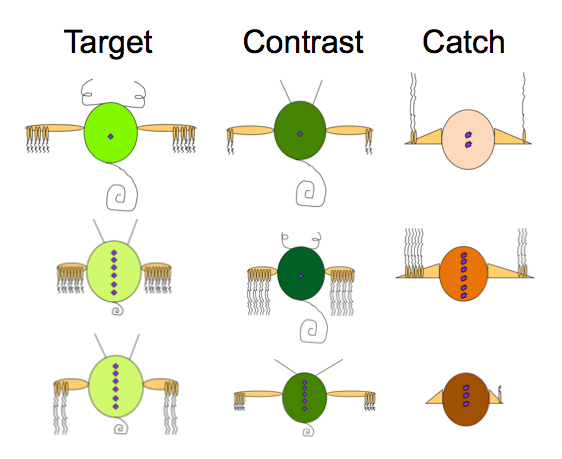
\includegraphics[scale=0.5]{bug_examples}
\caption[Example stimuli for supervised-sparse blocks]{Example stimuli for supervised-sparse blocks. Bugs varied on body color, tail size, wing length, number of fingers, finger length, dot number, and antennae shape.}
\vspace{-10pt}
\label{bugs}
\end{center}
\end{figure}

\begin{figure}[H]
\begin{center}
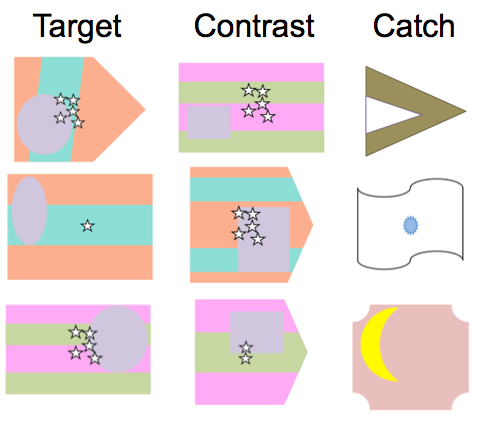
\includegraphics[scale=0.4]{flag_examples}
\caption[Example stimuli for unsupervised-sparse blocks]{Example stimuli for unsupervised-sparse blocks. Flags varied on shape, color, stripe direction, number of stars, overlay shape, overlay position, and overlay size.}
\vspace{-10pt}
\label{flags}
\end{center}
\end{figure}

\subsubsection{Dense stimuli}

\begin{figure}[H]
\begin{center}
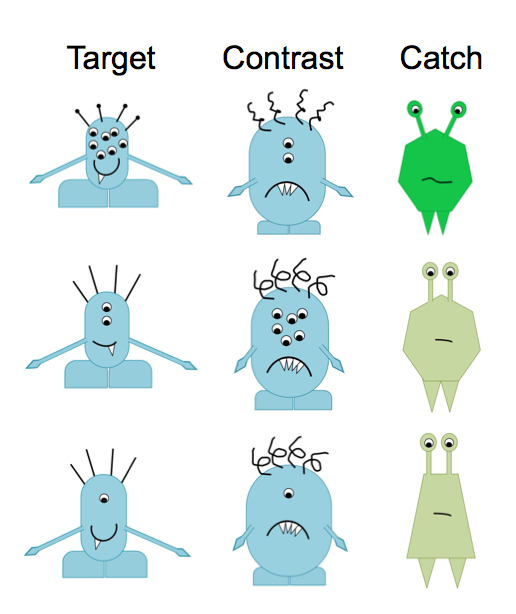
\includegraphics[scale=0.4]{alien_examples}
\caption[Example stimuli for unsupervised-dense blocks]{Example stimuli for unsupervised-dense blocks. Aliens varied on body size, arm length, foot size, number of teeth, smiling/frowning, hair shape, and number of eyes.}
\vspace{-10pt}
\label{aliens}
\end{center}
\end{figure}

\begin{figure}[H]
\begin{center}
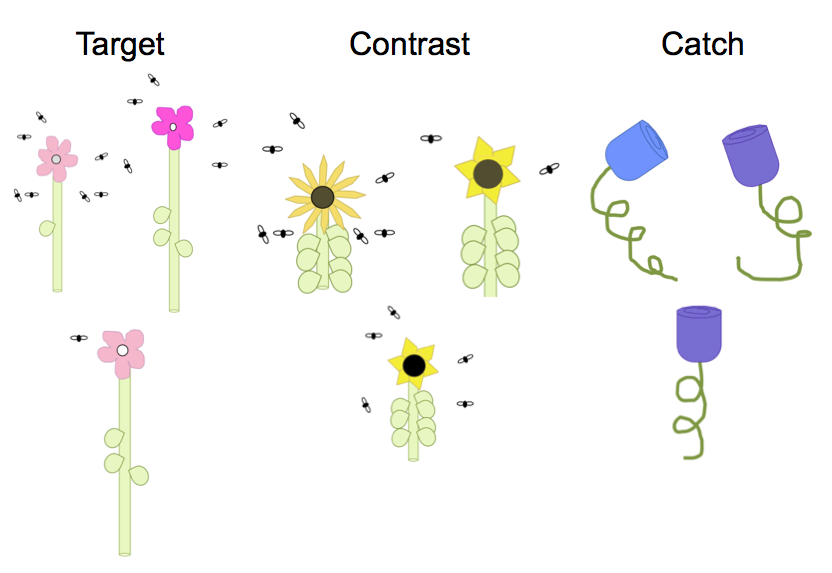
\includegraphics[scale=0.4]{flower_examples}
\caption[Example stimuli for supervised-dense blocks]{Example stimuli for supervised-dense blocks. Flowers varied on petal shape, petal color, stem length, number of leaves, center size, center color, and number of bugs.}
\vspace{-10pt}
\label{flowers}
\end{center}
\end{figure}

\subsection{Taxonomic/thematic task}

In the taxonomic/thematic task, participants saw a target item had to choose either a taxonomically- or thematically-related item. There were unrelated distractors as well as distractors with the opposite relation.

\subsubsection{Taxonomic version}

\begin{table}[H]
\caption{Stimuli for the taxonomic version.}
\vspace{-10pt}
\begin{center}
\begin{tabular}{cccc}
\toprule
Target & Taxonomic answer & Thematic distractor & Unrelated distractor \\
\midrule
Kettle & Coffee maker & Stove & Doorknob \\
Bird & Turtle & Tree & Guitar \\
Lock & Handcuffs & Key & Grapes \\
Sock & Pants & Shoe & Cake \\
Toaster & Microwave & Bread & Trumpet \\
Car & Train & Stop sign & Yarn \\
Airplane & Canoe & Neck pillow & Duck \\
Anchor & Weight & Life jacket & Antelope \\
Bat & Racket & Ball & Dresser \\
Binoculars & Microscope & Puffin & Bell \\
Blackboard & Easel & Ruler & Food processor \\
Cheese & Ice cream & Cheese grater & Chessboard \\
Chipmunk & Cat & Peanut & Mixer \\
Cigarette & Pipe & Cigarette cutter & Tissue box \\
Corkscrew & Peeler & Wine & Peanut \\
Cup & Mug & Juice & Ironing board \\
Eggs & Croissant & Pan & Ribbon \\
Fork & Spoon & Plate & Purse \\
Headband & Scrunchie & Hairbrush & Golf ball \\
Horn & Clarinet & Music stand & Chips \\
Knife & Sword & Cutting board & Camel \\
Lamp & Candle & Table & Mailbox \\
Mop & Duster & Bucket & Calculator \\
Motorcycle & Car & Helmet & Umbrella \\
Necklace & Ring & Jewelry box & Salt shaker \\
Paintbrush & Pen & Easel & Rooster \\
Printer & Shredder & Desk & Wheelchair \\
Soda & Juice & Chips & Seashell \\
String & Yarn & Sewing machine & Watch \\
Suitcase & Basket & Suit & Snow globe \\
\bottomrule
\end{tabular}
\label{taxstim}
\end{center}
\end{table}

\newpage

\subsubsection{Thematic version}

\begin{table}[H]
\caption{Stimuli for the thematic version.}
\vspace{-10pt}
\begin{center}
\begin{tabular}{cccc}
\toprule
Target & Thematic answer & Taxonomic distractor & Unrelated distractor \\
\midrule
Kettle & Stove & Coffee maker & Doorknob \\
Bird & Tree & Turtle & Guitar \\
Lock & Key & Handcuffs & Grapes \\
Sock & Shoe & Pants & Cake \\
Toaster & Bread & Microwave & Trumpet \\
Car & Stop sign & Train & Yarn \\
Strainer & Pasta & Peeler & Receipt \\
Axe & Log & Shovel & Thimble \\
Ladder & Lightbulb & Stool & Tire \\
Dog & Leash & Cat & Hair dryer \\
Exercise bench & Dumbbell & Exercise bike & Goggles \\
Cooler & Diet coke & Fridge & Camera \\
Corkscrew & Cork & Bottle opener & Globe \\
Gun & Bullet & Starfish & Sword \\
Money & Cash Register & Coin & Lunchbox \\
Parrot & Bird Cage & Butterfly & Skates \\
Candle & Lighter & Lantern & Clock \\
Suit & Hanger & Skirt & Scissors \\
High chair & Cup & Stroller & Button \\
Backpack & Binder & Purse & Balloon \\
Vacuum & Rug & Duster & Fish hook \\
Laundry basket & Shirt & Basket & Slinky \\
Wine glass & Wine bottle & Shot glass & Mirror \\
File cabinet & File & Dresser & Light switch \\
Steak & Grill & Ham & Remote \\
Doll & Dollhouse & Army man & Kayak \\
Roller blades & Helmet & Skateboard & Lawnmower \\
Record player & Speakers & Radio & Lipstick \\
Teeth & Toothbrush & Hair & Flashlight \\
Pie & Stove & Croissant & Crib \\
\bottomrule
\end{tabular}
\label{themstim}
\end{center}
\end{table}

\end{document}
